In this section, we discuss a running example extracted from the c base-class library with
challenges of computing the symbolic
\emph{reachability-bound} on
every control location and illustrate how our algorithm leverages the challenges through the \emph{path reachability-bound} and the \emph{loop reachability-bound}.
% This example
% % is adopted from the example in~\cite{GulwaniZ10}, which
% is a skeleton code extracted from the c base-class library.

% \paragraph{Challenges.}
\begin{example}
  [The Running Example with Two Paths Loop and Nested Loop in One Path]
  \label{ex:relatedNestedWhileOdd_abscfg}
    { \small
  \begin{figure}
  \centering
  \begin{subfigure}{.4\textwidth}
    \begin{centering}
    {\small
    $
    \begin{array}{l}
      \kw{nestedOdd}(n, m) \triangleq \\
      \clabel{ \assign{i}{n} }^{0} ; \\
          \ewhile ~ \clabel{i > 0}^{1} ~ \edo ~ \\
          \qquad \Big(
            \eif(\clabel{i \% 2 \neq 0 }^{2},\\
            \qquad \clabel{\assign{k}{i - m}}^{3};\\
            \qquad \ewhile ~ \clabel{k > 0}^{4} ~ \edo ~
            \Big( \clabel{\assign{k}{k - 1}}^{5} \Big);\\
            \qquad \clabel{\assign{i}{k + m}}^{6};
            \clabel{\assign{i}{i - 1}}^{7}, \\
            \qquad \clabel{\assign{i}{i - 3}}^{8})
            \Big)
      \end{array}
    $
    }
    \caption{}
    \end{centering}
    \end{subfigure}
  \begin{subfigure}{.5\textwidth}
    \begin{centering}
  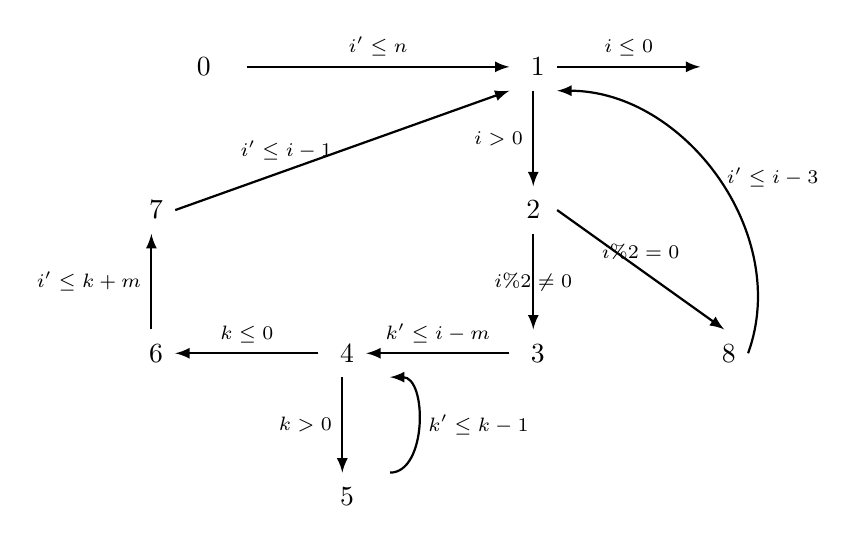
\begin{tikzpicture}[scale=\textwidth/20cm,samples=200]
  \draw[] (-7, 10) circle (0pt) node{{ $0$}};
  \draw[] (0, 10) circle (0pt) node{{ $1$}};
  \draw[] (0, 7) circle (0pt) node{\textbf{$2$}};
  \draw[] (0, 4) circle (0pt) node{{ $3$}};
  \draw[] (-4, 4) circle (0pt) node{{ $4$}};
  \draw[] (-8, 4) circle (0pt) node{{ $6$}};
  \draw[] (-4, 1) circle (0pt) node{{ $5$}};
  \draw[] (4, 4) circle (0pt) node{{ $8$}};
  \draw[] (-8, 7) circle (0pt) node{{ $7$}};
  % Counter Variables
  \draw[] (4.5, 10) circle (0pt) node {\textbf{$\lex$}};
  % \draw[] (6, 4) circle (0pt) node {{ $ex$}};
  %
  % Control Flow Edges:
  \draw[ thick, -latex] (-6, 10)    -- node [above] {\scriptsize $i' \leq n$}(-0.5, 10);
  \draw[ thick, -latex] (0, 9.5)    -- node [left] {\scriptsize $i > 0$} (0, 7.5) ;
  \draw[ thick, -latex] (0.5, 7)    -- node [above] {\scriptsize $ i \% 2 = 0 $}  (4, 4.5);
  \draw[ thick, -latex] (4.5, 4)    to  [out=70,in=0]   node [right] {\scriptsize $i' \leq i - 3$ }(0.5, 9.5);
  \draw[ thick, -latex]  (0, 6.5)   -- node  {\scriptsize $i \% 2 \neq 0$}  (0, 4.5) ;
  \draw[ thick, -latex]  (-0.5, 4)  -- node [above] {\scriptsize $k' \leq i - m$ }  (-3.5, 4) ;
  \draw[ thick, -latex]  (-4.5, 4)  -- node [above] {\scriptsize $k \leq 0$ }  (-7.5, 4);
  \draw[ thick, -latex] (0.5, 10)   -- node [above] {\scriptsize $i \leq 0$}  (3.5, 10);
  \draw[ thick, -latex] (-4, 3.5)   -- node [left] {\scriptsize $k > 0$}  (-4, 1.5);
  \draw[ thick, -latex] (-3, 1.5)   to  [out=0,in=0] node [right] {\scriptsize $k' \leq k- 1$}  (-3, 3.5);
  \draw[ thick, -latex] (-8, 4.5)   --  node [left] {\scriptsize $i' \leq k + m$ }(-8, 6.5);
  \draw[ thick, -latex] (-7.5, 7)  --  node [left] {\scriptsize $i' \leq i - 1$ }(-0.5, 9.5);
  % \draw[ thick, -latex] (6, 6.5)  -- node [right] {$\top$} (6, 4.5) ;
  \end{tikzpicture}
  \caption{}
    \end{centering}
    \end{subfigure}
\begin{subfigure}{.9\textwidth}    
\begin{centering}
  {\small
  $\tpath_0 = (0 \to 1)$
  \quad
  $\tpath_1 = (1 \to 2 \to 3 \to 4)$
  \quad
  $\tpath_2 = (4 \to 6 \to 7 \to 1)$
  \quad
  $\tpath_3 = (4 \to 5 \to 4)$
  \quad
  $\tpath_4 = (1 \to 2 \to 8 \to 1)$
  \quad
  $\tpath_5 = (1 \to \lex)$
  \\
  $
  \tpath_0 ; \rpchoose{ 1: \rprepeat(\tpath_1; 4:\rprepeat(\tpath_3); \tpath_2; \tpath_4), 
  1: \rprepeat(\tpath_4; \tpath_1; 4:\rprepeat(\tpath_3); \tpath_2) }; \tpath_5
  $
  }
  % \caption{}
    \end{centering}
    \end{subfigure}
  \caption{
  (a) The program of the two paths loop with a nested Loop in one path,
    (b) The corresponding \emph{Abstract Transition Graph}, $\absG(\kw{nestedOdd}(n, m))$. }
      \label{fig:relatedNestedWhileOdd-overview}
  \end{figure}
  }
  %
  \end{example}    
  
% \todo{Shorten}
% \begin{itemize}
% \item 
\textbf{Challenge I}
The example program in Figure~\ref{ex:relatedNestedWhileOdd-overview}(a) has two level nested loops, outer loop $L_1$ and nested loop $L_4$ which is in the first path of $L_1$. Given $n \geq m \geq 0$,
the expected \emph{reachability-bound}s for locations in outer loop $3, 6, 7$ and $8$ are all $\lfloor\frac{m}{4}\rfloor$,
% for $8$ is $\lfloor\frac{m}{4}\rfloor + 1$,
for location $2$ is $\lfloor\frac{m}{2}\rfloor$ and $\lfloor\frac{m}{2}\rfloor + 1$ for location $1$.
\highlight{Though within the same loop $L_1$, the bounds for different locations are different.}
The amortized analysis methodology such as Loopus~\cite{SinnZV17}, KoAT~\cite{BrockschmidtEFFG14,FalkeKS12,FalkeKS11}, C4B~\cite{CarbonneauxHS15}, etc. ignores path sensitivity and approximate the bound $n$ as the bound for loop $L_1$. 
While some path-refinement-based methods such as \cite{GulwaniZ10,GulwaniJK09}, CoFloCo~\cite{Montoya17,Flores-Montoya16,Flores-MontoyaH14} and etc. only give the same bound for all the locations within the loop $L_1$. 
Though we can reuse their results i.e., loop bounds as the \emph{reachability-bound} for location $1$ and $2$,
but it is still unclear for locations $3, 6, 7$, and $8$.
%
This motivates our first key novelty -- the \emph{path reachability-bound} $\inoutB(\rprog, \tpath)$ for a loop-free and interleaving-free path $\tpath$.
It bounds the evaluation times of each path over a path-refined program.
% \item 

\textbf{Challenge II} The second challenge occurs in the nested loop.
In line 6, since $i$ is reset by $k + m$ and $k$ is reset by $i - m$ at line 3, the
loop $L_4$ is only executed in the first iteration of while loop $L_1$.
% \\
The total iterations of the two loops are
$n - m + \lfloor\frac{m}{2}\rfloor + 1$,
and the tight \emph{reachability-bound} for location $5$ inside the $L_4$ is $m$.
% for locations $4, 5$ and $8$ between the $L_3$ and $L_6$ are $(n-N) \times (m - N)$,
% and $n - N$ for locations $2$ and $9$.
% \\
\highlight{The tight \emph{reachability-bound}s for the locations inside the loop $L_4$ is 
the same as its innermost loop iteration bound.
% , as well as our \emph{path reachability-bound}.
However, for the locations between $L_1$ and $L_4$,
the tight bounds are the multiplication of the inner and outer loop iteration bounds.}
% \\
% compute a better but still loose bound, $n + m^2 - m \times N$ on total iteration times.
The existing approach either ignores the path sensitivity or computes the same bound for all the locations in a loop.
None of them can give the precise \emph{reachability-bound}s for different locations in the loop,
which is non-trivial to compute even though knowing the loop bound.
% especially for the locations similar to $7$ in $\kw{threeNestedWhile}$.
This motivates us to consider our second novel quantity --
the numbers of iterations of the outer loop $L_1$ such that,
during these iterations, the loop $L_4$ is ``entered''. 

We refer to this quantity as the \emph{loop reachability} of the loop $L_4$ w.r.t the outer loop $L_1$.
% of the location within loop $L_6$ w.r.t the loops $L_3$ and $L_1$.
By multiplying the \emph{path reachability-bound} of $\tpath_3$ within $L_4$,
with its \emph{loop reachability-bound} w.r.t $L_1$, we can obtain an accurate
\emph{reachability-bound} for location $5$.
This quantity isn't considered or computed in any of the previous works.
\cite{GulwaniJK09} considers a similar quantity, the \emph{Progress Invariant}. But it bounds the iteration times of inner loop $L_4$ w.r.t. one iteration of $L_1$, which is $m$. Then they still over-approximate the bound for locations inside $L_4$ as $m \times (n - m)$ by multiplication.
% \end{itemize}
With the two key novelties, our algorithm computes the reachability-bound for this example through the following steps.

\textbf{\emph{Step1: Program abstraction.}}
In Section~\ref{sec:progabs},
we first 
generate the \emph{Abstract Transition Graph} as in Figure~\ref{fig:relatedNestedWhileOdd-overview}(b).
Each edge $l \xrightarrow{dc} l'$ is an abstract transition $\absevent = (l, dc, l')$ annotated with a constraint $dc$ corresponding to the command of label $l$.

Then we abstract the program in the form of paths.
$$
\tpath_0 ; \rpchoose{ 1: \rprepeat(\tpath_1; 4:\rprepeat(\tpath_3); \tpath_2), 1:\rprepeat(\tpath_4) }; \tpath_5
$$
$;$ concatenates sequence of execution paths,
$\rprepeat(\tpath_3)$ represents looping on the path $\tpath_3$ and
$\rpchoose{ \ldots}$ represents the loop $L_1$ which contains two possible execution paths,
$\rprog_1 = \tpath_1; 4:\rprepeat(\tpath_3);\tpath_2$ and $\rprog_2 =\tpath_4$.

% \textbf{Step 2: Program Refinement}
\textbf{\emph{Step 2: Path interleaving refinement.}} 
Two execution paths are not simply iterating on themselves during the program execution,
they could interleave each other at certain iteration.
We summarize each execution path into conjunctions of transition relations.
\begin{equation}
    \begin{array}{l}
        \rprog_1 \models \phi_1 = \\
    \rprog_2 \models \phi_2 = 
    \end{array}
\end{equation}
  
In this sense, Algorithm~\ref{alg:prog-refine} in Section~\ref{sec:refine} computes the interleaving orders
by exhaustively checking the compositions of transition relations of different execution paths,
\begin{equation}
    \begin{array}{l}
        \rprog_1 ; \rprog_1 \models \exists i, k \st \phi_1 \circ \phi_1 = ... \implies \efalse\\
        \rprog_2 ; \rprog_2 \models \exists i, k \st \phi_2 \circ \phi_2 = ... \implies \efalse \\
        \rprog_2 ; \rprog_1 \models \exists i, k \st \phi_2 \circ \phi_1 = ...  \\
        \rprog_1 ; \rprog_2 \models \exists i, k \st \phi_1 \circ \phi_2 = ... 
    \end{array}
\end{equation}
Only two execution paths are feasible, so we identify two unique interleaving orders --
either $\rprog_1$ executes after one iteration of $\rprog_2$ or vice versa.
% Then, loop $L_1$ in the source program is generates new execution paths as follows,
\[
    \rprog^1 = \rprog_1 ; \rprog_2 = \tpath_1; 4:\rprepeat(\tpath_3); \tpath_2; \tpath_4
    \qquad
    \rprog^2 = \rprog_2 ; \rprog_1 = \tpath_4; \tpath_1; 4:\rprepeat(\tpath_3); \tpath_2
\]
% The second step in Section~\ref{sec:refine}
Then, the multiple-paths loop $L_1$ in the source program is refined
into multiple loops where each one can only iterate following the specified interleaving order.
% the interleaving of paths is explicit.
As in the bottom of Figure~\ref{fig:relatedNestedWhileOdd-overview}(c),
the program is transformed into 
\[
    \tpath_0 ; \rpchoose{ 1: \rprepeat(\tpath_1; 4:\rprepeat(\tpath_3); \tpath_2; \tpath_4), 
1: \rprepeat(\tpath_4; \tpath_1; 4:\rprepeat(\tpath_3); \tpath_2) }; \tpath_5
\]
In this refined program, 
each new execution path is equivalent to the execution of the original loop. 
% denoted as $\rprog_1^1$ and $\rprog_1^2$.

% \textbf{Step 3: Ranking Function Estimation}
\textbf{\emph{Step 3: ranking function estimation.}}
Algorithms in Section~\ref{sec:rank} identifies the ranking function for each transition edge, which is a symbol whose number of decreasing times can represent the number of execution of this edge.
For example for edge $4 \to 5$, its ranking function is $k$ and edges on $\tpath_1$, $\tpath_2$ and $\tpath_4$ all have $i$ as their ranking functions.

% \textbf{Step 4: Path-sensitive Reachability-bound Computation.}
\textbf{\emph{Step 4: local path reachability-bound.}}
For $\tpath_3$ in the program in Figure~\ref{fig:relatedNestedWhileOdd-overview}, we want to know how many times it is ``reached'' during the program execution.
From the refined program, $\tpath_3$ shows up in both newly generated execution paths $\rprog^1$ and $\rprog^2$  and nested in two level loops.
The algorithm in Section~\ref{sec:pathlocalrb} first
% computes a local \emph{path reachability-bound} for it w.r.t. its innermost loop $L_4$ by computing 
computes three abstract states for the ranking functions on $\tpath_3$ when first, second and last visiting during execution of $L_4$,
\begin{equation*}
    \rfinit(\rprog^1, \tpath_3, c) = \{k = n - m\} \quad
    \rfnext(\rprog^1, \tpath_3, c) = \{k = 1\} \quad
    \rffinal(\tpath_3, c) = \{ k = 0 \}.
\end{equation*}
Then  the maximal value of the following formula provides   
an upper bound on the number of execution times of $\tpath_3$ when executing only the innermost loop where $\tpath_3$ is nested. 
\[
    \max
    \left\{ 
        {\frac{a - b}{1}} 
        ~\vert~
        x = a \in \{k = n - m\}
        \land x = b \in \{ k = 0 \}
    \right\}  = n - m
\]
% The algorithm in Section~\ref{sec:pathlocalrb}
% computes $\outinB(4:\rprepeat(\tpath_3), \tpath_3, c) = n - m$ by computing
% the initial state, next state and final state of ranking functions on $\tpath_3$ during the execution of $\rprepeat(\tpath_3)$.

\textbf{\emph{Step 5: loop reachability-bound.}}
Previous step only provides the path reachability-bound for a simple transition path w.r.t. the innermost loop.
For nested loops, we need to compute the \emph{loop reachability-bound} for each simple transition path with respect to every level of the outer loop.
Since $\tpath_3$ is nested in two level loops, we compute its \emph{loop reachability-bound}
with respect to the outer loop $L_1$. 
It is expected to be $1$ because the inner loop $L_4$ is reached only in the first iteration of the outer loop $L_1$.
% , we aim to compute $1$ as the \emph{loop reachability-bound} of $\tpath_3$ w.r.t. $L_1$.
In the first refined execution path, $\rprog^1 = \rprepeat(\tpath_1; 4:\rprepeat(\tpath_3); \tpath_2; \tpath_4)$,
we compute three abstract states when visiting $L_4$ the first, second and last time during the execution of loop $\rprog^1$,
\begin{equation*}
\lpinit(\rprog^1, \tpath_3, c) = \max\{ n - m\} \quad
\lpnext(\rprog^1, \tpath_3, c) = \max\{n - m\} \quad
\rffinal(\tpath_3, c) = \{k = 0\}.
\end{equation*}
Then we compute \emph{loop reachability-bound} as the maximal value of the formula,
\[
    \max\limits_{x = a \in \{k = 0\}}
    \frac{\lpinit(\max\{n - m\} - a }{\max\{n - m\}} = 1
  \]
We also compute in the second refined execution path $\rprog_1^2$ the same number.
% $\outinB(4:\rprepeat(\tpath_3), \tpath, c) = n - m - 3$ and the same $\lpchB(\rprog_1^2, \tpath_3, c)$.
% So 

\textbf{\emph{Step 6: path reachability-bound.}}
For each simple transition path in every refined execution path where it shows up, we take the production of the \emph{loop reachability-bound}
and local \emph{path reachability-bound}.
For example for $\tpath_3$ in the first refined execution path 
$\rprepeat(\tpath_1; 4:\rprepeat(\tpath_3); \tpath_2; \tpath_4)$,
we compute $1 \times (n - m)$ and $1 \times (n - m - 3)$ in the second execution path.
Then we
take the maximal value over all refined execution order and
$\inoutB(\rprog, \tpath_3, c) = \max\{ 1 \times (n - m), 1 \times (n - m - 3) \} = n - m$.
This maximization operation does not produce over-approximation because there does not exist interleave
between the refined execution paths and each refined execution path is equivalent to the original loop, and each other as well.

\textbf{\emph{Step 7: reachability-bound.}}
Now for every program point $l$, we sum up the $\inoutB(\rprog, \tpath)$ over all $\tpath$ that contains $l$ and get $\psRB(l, c)$.
Since point $5$ only shows up on $\tpath_3$, we compute \highlight{$\psRB(5, c) = n - m$}.
The points $0$ and $\lex$ are not in any loop, so we have $\psRB(0, c) = \psRB(\lex, c) = 1$.
The points $3, 6, 7$ and $8$ which only show up once on $\tpath_2$ and $\tpath_4$ are all equal to $\lfloor\frac{m}{4}\rfloor$ the same as their $\inoutB$.
For the loop headers $1$ and $4$, we only count the $\tpath$ where they show up as a start-point.
So $\psRB(4, c) = \lfloor\frac{m}{4}\rfloor + n - m + 1$ and $\psRB(1,c) = 2 \times \lfloor\frac{m}{4}\rfloor + 1$ all as expected.